\section{ZLP subtraction and bandgap determination in WS$_2$}
\label{sec:results_sample}

Following the discussion of the vacuum ZLP analysis, we now
present the application of our machine learning strategy to parametrise the ZLP
arising in EEL spectra recorded on specimens.
%
Specifically, we will analyse EELS measurements acquired on different regions
of the WS$_2$ nanoflowers reviewed in Sect.~\ref{sec:tmd}.
%
The resulting ZLP parametrisation will then be used to isolate the inelastic
contribution $I_{\rm inel}$ in each spectrum and determine the bandgap energy $E_{\rm BG}$ from
its behaviour in the onset region.

\subsection{Training dataset}
%
Low-magnification TEM images of two representative regions of
the WS$_2$ nanoflowers are displayed in Fig.~\ref{fig:ws2positions},
denoted as sample A and sample B.
%
In each image we indicate the specific locations where
EEL spectra have been recorded, including in-vacuum measurements taken
for calibration purposes.
%
Note that in sample B  the differences in contrast are related to the material
thickness, with higher contrast corresponding to thinner regions.
%
The two samples exhibit different structural morphologies: while sample A is composed
by a relatively thick region of WS$_2$, sample B corresponds to a thin petal region
with possibly overlapping terraces.
%
In other words, sample A is composed by bulk WS$_2$ while in sample B some specific regions
could be rather thinner, down to the few monolayers level.
%
This thickness information has been be determined
by means of the {\tt Digital~Micrograph}  software.
%
Further, the measurements on each sample have
been obtained with different electron microscopes and
operation settings, and for this reason
we analyse them independently.

%%%%%%%%%%%%%%%%%%%%%%%%%%%%%%%%%%%%%%%%%%%%%%%%%%%%%%%%%%%%%%%%%%%%%%%
\begin{figure}[t]
\begin{centering}
  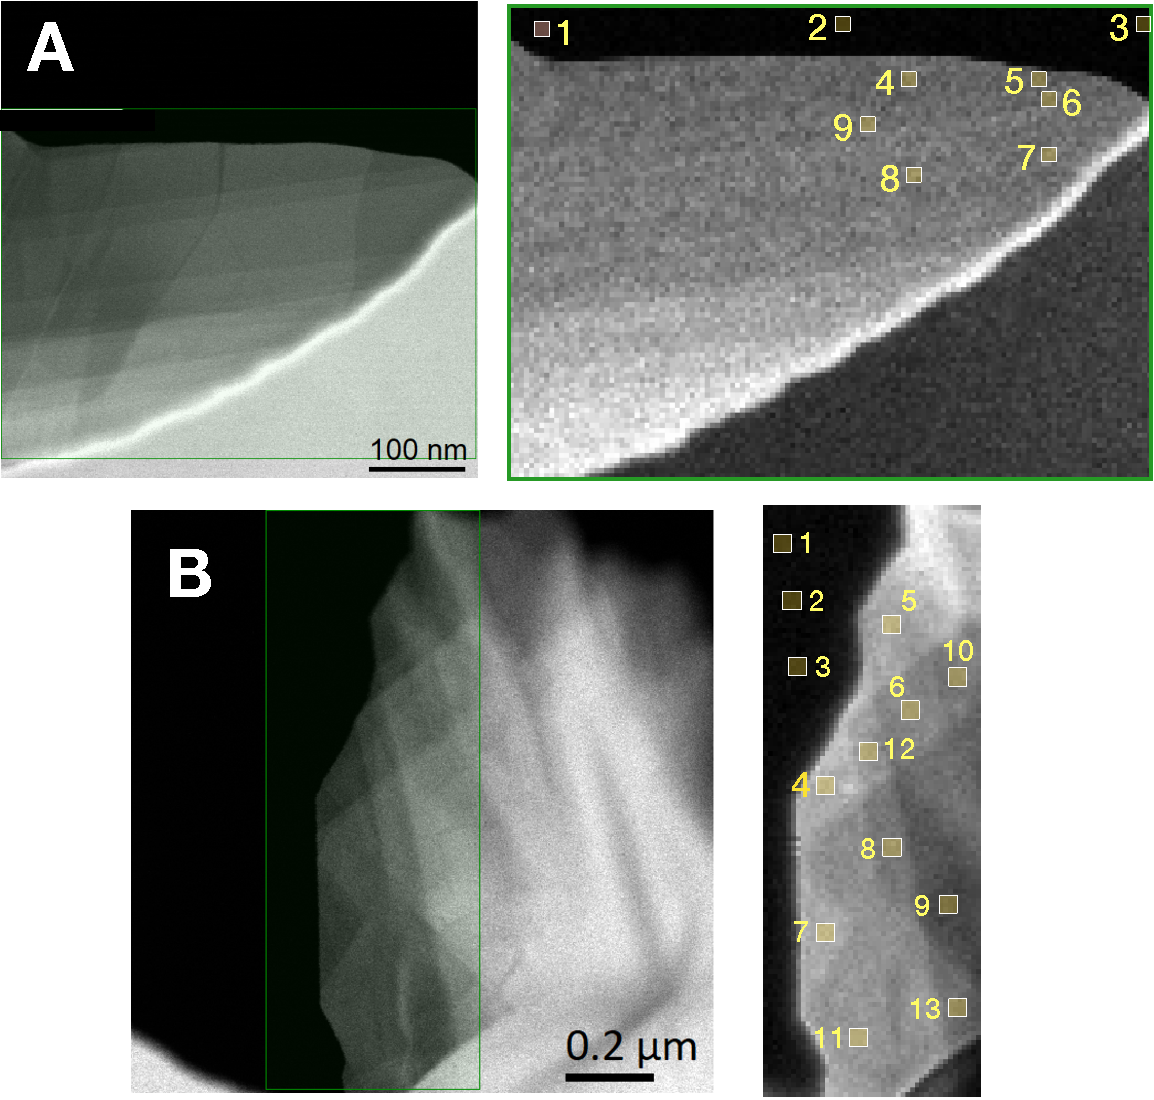
\includegraphics[width=0.87\linewidth]{plots/Spectra_location.pdf}
  \caption{Low-magnification TEM images of two different regions of
    the WS$_2$ nanoflowers, denoted as sample A and sample B respectively.
    %
    In each image we indicate the locations where
    EEL spectra have been recorded, including the in-vacuum measurements taken
    for calibration purposes.
    %
    In sample B the difference in contrast is correlated to the material
    thickness, with higher contrast corresponding to thinner regions of the nanostructure.
    %
    The morphological differences between the two samples are discussed in the text.
  }
\label{fig:ws2positions}
\end{centering}
\end{figure}
%%%%%%%%%%%%%%%%%%%%%%%%%%%%%%%%%%%%%%%%%%%%%%%%%%%%%%%%%%%%%%%%%%%%%%%%%%

In Table~\ref{table:sampledata} we collect the most relevant properties of the spectra collected
in the locations indicated in Fig.~\ref{fig:ws2positions} using the same format as
in Table~\ref{table:vacuumdata}.
%
Note that since the of spectra from samples A and B
have been acquired with different microscopes, features of the ZLP
such as the FWHM are expected to be different.
%
From this table one can observe how  the ZLP for the spectra acquired on sample A exhibit
a FWHM about three times higher as compared to those of sample B
than the resolution obtained on the second set. 
%
This difference can be understood from the fact that the EELS spectra from sample B, unless those
from sample B,
were recorded with a TEM equipped with a monochromator.

%%%%%%%%%%%%%%%%%%%%%%%%%%%%%%%%%%%%%%%%%%%%%%%%%%%%%%%%%%%%%%%%%%%%%%%%%%%%%%%%%%%%%%%%%%%%%
%%%%%%%%%%%%%%%%%%%%%%%%%%%%%%%%%%%%%%%%%%%%%%%%%%%%%%%%%%%%%%%%%%%%%%%%%%%%%%%%%%%%%%%%%%%%%
\begin{table}[t]
  \begin{center}
            \renewcommand{\arraystretch}{1.50}
  \begin{tabular}{@{}ccccccccc}
\br
Set & $t_{\rm exp}$ {(}ms{)} & $E_{\rm b}$ {(}keV{)} & $N_{\rm sp}$ & $N_{\rm dat}$ & $\Delta E_{\rm min}$~(eV)  & $\Delta E_{\rm max}$~(eV)  & FWHM~(eV)  \\ 
\mr
A        &       ?       &        ?         &   6      &    1918    &     -4.1       & 45.5 & $ 0.47\pm0.01$  \\
B        &       ?       &    200 keV       &   10     &    2000    &     -0.9        & 9.1   & $ 0.16\pm0.01$ \\
\br
  \end{tabular}
    \end{center}
  \caption{\small Same as Table~\ref{table:vacuumdata} now for the EEL spectra taken on specimens A and B.
    %
    Note that the location on the WS$_2$ nanoflowers where each spectra has been recorded
    was indicated in Fig.~\ref{fig:ws2positions}.
  }
   \label{table:sampledata}
\end{table}
%%%%%%%%%%%%%%%%%%%%%%%%%%%%%%%%%%%%%%%%%%%%%%%%%%%%%%%%%%%%%%%%%%%%%%%%%%%%%%%%%%%%%%%%%%%%%%%%%5
%%%%%%%%%%%%%%%%%%%%%%%%%%%%%%%%%%%%%%%%%%%%%%%%%%%%%%%%%%%%%%%%%%%%%%%%%%%%%%%%%%%%%%%%%%%%%

In the following we will present results for representative spectra
corresponding to each of the two samples.
%
The full set of spectra together are available together with {\tt EELSfitter},
the code used to produce the results of this analysis
and whose installation
and usage instructions are presented in Appendix~\ref{sec:installation}.


\subsection{Subtraction procedure}

In Table~\ref{table:sampledata_summary} we collect
the mean value and uncertainty of the first local minimum, $\Delta E|_{\rm min}$,
averaged over the spectra corresponding to samples A and B from
Fig.~\ref{fig:ws2positions},
as well as the corresponding values of the hyper-parameters
 $\Delta E_{\rm I}$ and $\Delta E_{\rm II}$ defined in Fig.~\ref{fig:EELS_toy}.
%
Recall that only
the data points with $\Delta E \le \Delta E_{\rm I}$ is used for the training
of the neural network model.
%
For $\Delta E \ge \Delta E_{\rm II}$ instead, the training set includes only the pseudo-data
that implements the $I_{\rm ZLP}(\Delta E)\to 0$ constraint.
%
 The location of the first minimum is relatively stable
 among all the spectra belonging to a given set.
 %
 This indicates that the onset of the inelastic contributions $I_{\rm inel}$ does
 not change significantly as we move to different regions of the sample.
 %
 The model training is performed for a range of $\Delta E_{\rm I}$ values
 subject to the condition that $\Delta E_{\rm I} \le \Delta E_{\rm min}$,
 with the optimal values listed  in Table~\ref{table:sampledata_summary} selected
 by comparing the intensity derivatives in the sample with the vacuum reference.

%%%%%%%%%%%%%%%%%%%%%%%%%%%%%%%%%%%%%%%%%%%%%%%%%%%%%%%%%%%%%%%%%%%%%%%%%%%%%%%%%%%%%%%%%%%%%
%%%%%%%%%%%%%%%%%%%%%%%%%%%%%%%%%%%%%%%%%%%%%%%%%%%%%%%%%%%%%%%%%%%%%%%%%%%%%%%%%%%%%%%%%%%%%
\begin{table}[t]
  \begin{center}
            \renewcommand{\arraystretch}{1.50}
  \begin{tabular}{@{}ccccccccc}
\br
Set & $\Delta E|_{\rm min}$~(eV)  &  $\Delta E_{\rm I}$~(eV)  &  $\Delta E_{\rm II}$~(eV)   \\
\mr
A        &    $2.70\pm0.06$               &          1.8        &      12         \\
B        &    $1.80\pm0.04$               &          1.4        &      6        \\
\br
  \end{tabular}
    \end{center}
  \caption{\small The mean value and uncertainty of the first local minima, $\Delta E|_{\rm min}$,
    averaged over the spectra corresponding to samples A and B from
    Fig.~\ref{fig:ws2positions}.
    %
    We also indicate
     the corresponding values of the hyper-parameters
     $\Delta E_{\rm I}$ and $\Delta E_{\rm II}$ defined in Fig.~\ref{fig:EELS_toy} used for the training
     of the neural network model.
    %
  }
   \label{table:sampledata_summary}
\end{table}
%%%%%%%%%%%%%%%%%%%%%%%%%%%%%%%%%%%%%%%%%%%%%%%%%%%%%%%%%%%%%%%%%%%%%%%%%%%%%%%%%%%%%%%%%%%%%%%%%5
%%%%%%%%%%%%%%%%%%%%%%%%%%%%%%%%%%%%%%%%%%%%%%%%%%%%%%%%%%%%%%%%%%%%%%%%%%%%%%%%%%%%%%%%%%%%%

The result of the  neural network training is
 a set of $N_{\rm rep}=500$ replicas
  parametrising the ZLP, $I_{\rm ZLP}^{({\rm mod})(k)}(\Delta E)$.
 %
 Taking into account that we have $N_{\rm sp}$ individual spectra in each sample,  the ZLP
 subtraction is performed individually
 for each Monte Carlo replica,
 \be
 \label{eq:subtractedModelPrediction}
 I_{\rm inel}^{({\rm exp})(j,k)}(\Delta E) \equiv I_{\rm EELS}^{({\rm exp})(j)}(\Delta E) - I_{\rm ZLP}^{({\rm mod})(k)}(\Delta E)\, ,
 \quad \forall~N_{\rm rep} \, ,\quad j=1,\ldots,N_{\rm sp} \, ,
 \ee
 from which statistical estimators can be evaluated as usual.
 %
 For instance, the mean value for our model prediction for the $j$-th spectrum
 can be evaluated by averaging over the set of replicas,
 \be
 \la  I_{\rm inel}^{({\rm exp})({\rm (exp)}j)}\ra (\Delta E)
 = \frac{1}{N_{\rm rep}} \sum_{k=1}^{N_{\rm rep}}  I_{\rm inel}^{({\rm mod})(j,k)}(\Delta E) \, ,
 \quad j=1,\ldots,N_{\rm sp} \, ,
 \ee
 and likewise for the corresponding uncertainties or correlations.
%
 For large values of $\Delta E$
 the model prediction reduces to the original spectra, since in that region
 the ZLP contribution vanishes,
 \be
 I_{\rm inel}^{({\rm exp})(j,k)}(\Delta E \gg \Delta E_{\rm I}) \to  I_{\rm EE}^{{\rm (exp)}(j)}(\Delta E) \, ,\quad
 \forall~j,k \, .
 \ee
 
 For very small values of the energy loss, the contribution to the total
 spectra from inelastic scatterings is negligible
 and thus the subtracted model prediction Eq.~(\ref{eq:subtractedModelPrediction}) should
 vanish.
 %
 However, this will not be the case in practice since the neural-net model is trained on
 the $N_{\rm sp}$ ensemble of spectra, rather that just on individual ones, and thus the expected
 $\Delta E \to 0$ behaviour will only be achieved within uncertainties rather than at the level of
 central values.
 %
 To achieve the desired $\Delta E \to 0$ limit, we apply a matching procedure
 as follows.
 %
 We introduce another hyper-parameter, $\Delta E_0 < \Delta E_1$, such that
 one has for the $k$-th ZLP replica associated to the $j$-th spectrum the following
 behaviour:
 \bea
 \nonumber
 I_{\rm ZLP}^{({\rm mod})(j,k)}(\Delta E) &=& I_{\rm EELS}^{({\rm exp})(j)}(\Delta E) \, ,\quad \Delta E < \Delta E_0  \, ,\\
 I_{\rm ZLP}^{({\rm mod})(j,k)}(\Delta E) &=& I_{\rm EELS}^{{\rm (exp)}(j)} + \lp \xi_1^{(n_l)(k)}(\Delta E) -
 I_{\rm EELS}^{{\rm (exp)}(j)}(\Delta E)\rp  \times \mathcal{F} \, , \nonumber \quad 
 \Delta E_0 < \Delta E \le \Delta E_1 \, ,\\
 &&\mathcal{F} = \exp\lp -\frac{\lp \Delta E - \Delta E_1 \rp^2 }{\lp \Delta E_0 - \Delta E_1 \rp^2 \delta^2} \rp  \, , \label{eq:matching} \\
 I_{\rm ZLP}^{({\rm mod})(j,k)}(\Delta E) &=& \xi_1^{(n_l)(k)}(\Delta E) \, , \quad \Delta E > \Delta E_1 \nonumber \, ,
 \eea
 where $\xi_1^{(n_l)(k)}$ indicates the output of the $k$-th neural network that parametrises
 the ZLP and $\delta$ is a dimensionless tunable parameter.
 %
 In Eq.~(\ref{eq:matching}), $\mathcal{F}(\Delta E)$ represents a matching factor
 that ensures that the ZLP model prediction smoothly interpolates
 between $\Delta E=\Delta E_0$ (where $\mathcal{F}\ll 1$ and the original spectrum should
 be reproduced) and $\Delta E=\Delta E_1$
 (where $\mathcal{F}=1$ leaving the neural network output unaffected).
 %
 Here we adopt $\Delta E_0 = \Delta E_1 -0.5\,{\rm eV}$,  having verified
 that results are fairly independent of this choice.
 %
 Taking into account the matching procedure, we can slightly modify Eq.~(\ref{eq:subtractedModelPrediction})
 to 
 \be
 \label{eq:subtractedModelPrediction2}
 I_{\rm inel}^{({\rm mod})(j,k)}(\Delta E) \equiv I_{\rm EELS}^{({\rm exp})(j)}(\Delta E) - I_{\rm ZLP}^{({\rm mod})(j,k)}(\Delta E)\, ,
 \quad \forall~N_{\rm rep} \, ,\quad j=1,\ldots,N_{\rm sp} \, .
 \ee

 The ensemble of ZLP-subtracted spectra $\{I_{\rm inel}^{({\rm mod})(j,k)} \} $
 can then be used to estimate the bandgap of the specimen in the region where
 they were acquired.
 %
 Different approaches  have been put forward to estimate the value of the bandgap from 
subtracted EEL spectra, \textit{e.g.} by means of the inflection point of the rising intensity or
a linear fit to the maximum positive slope~\cite{Schamm:2003}.
%
Here we will adopt the approach of~\cite{Rafferty:2000} where the behaviour
of $I_{\rm inel}(\Delta E)$ in the onset region is modeled as
\begin{equation}
  \label{eq:I1}
    I_{\rm inel}(\Delta E) \simeq  A \lp \Delta E-E_{\rm BG} \rp^{b} \, , \quad \Delta E \ge E_{\rm BG} \, ,
\end{equation}
and vanishes for $E < E_{\rm BG}$, where both the bandgap value
$E_{\rm BG}$ as well as the parameters $A$ and $b$ are extracted from the fit.
%
The exponent $b$ is expected to be $b\simeq 1/2~(3/2)$ for a semiconductor material characterised
by a direct~(indirect) bandgap.
 %
 For each of the $N_{\rm sp}$ spectra and the $N_{\rm rep}$ replicas
 we fit to Eq.~(\ref{eq:subtractedModelPrediction2}) the model Eq.~(\ref{eq:I1})
 within a range taken to be
 $\lc \Delta E_{\rm I} - 0.5~{\rm eV}, \Delta E_{\rm I} + 0.7~{\rm eV}\rc$.
 %
 One ends up with $N_{\rm rep}$ values for
 the bandgap energy and fit exponent for each spectra,
 \be
 \Big \{ E_{\rm BG}^{(j,k)}, b^{(j,k)} \Big\} \, , \quad k=1,\ldots,N_{\rm rep} \, ,
 \quad j=1,\ldots,N_{\rm sp} \, ,
 \ee
 from which again one can readily evaluate their statistical estimators.
 %
 In the following, we will display the median and the 68\% confidence level intervals
 in these parameters to account for the fact distributon in in general non-gaussian.

 \subsection{Bandgap analysis of sample A}

 We present first the results of the bandgap analysis of sample A,
 taking sp14 as representative spectrum.
 %
 The left panel of Fig.~\ref{fig:sp4_subtracted_spectrum} displays the original
  and subtracted EEL spectrum corresponding to location sp14 of sample A in Fig.~\ref{fig:ws2positions},
  together with the predictions of the ZLP model.
  %
  The bands indicate the 68\% CL uncertainties.
  %
  The inset displays the result of the fit using Eq.~(\ref{eq:I1}) to the onset
  region of the subtracted spectrum.

  
  
Both for the ZLP model and for the subtracted spectrum we show both the central value
and the standard deviation of the predictions.
%
One can observe how uncertainties are negligible at low $\Delta E$
(due to the matching condition) and large $\Delta E$ (where the ZLP vanishes).
%
It is also possible to verify {\it a posteriori} that the choice of $\Delta E_I$
is sensible, by evaluating the following ratio
\be
\mathcal{R}_{\rm abs}\lp \Delta E_1\rp \equiv 
\la I_{\rm ZLP}^{({\rm mod})(j)}\ra /I_{\rm EELS}^{(j)} \Big|_{\Delta E = \Delta E1} \, .
\ee
One should verify that $\mathcal{R}_{\rm abs}\lp \Delta E_1\rp$ is not too far from unity,
indicating that the training dataset has not been contaminated by the inelastic contributions.
     
%%%%%%%%%%%%%%%%%%%%%%%%%%%%%%%%%%%%%%%%%%%%%%%%%%%%%%%%%%%%%%%%%%%%%%%
\begin{figure}[t]
\begin{centering}
  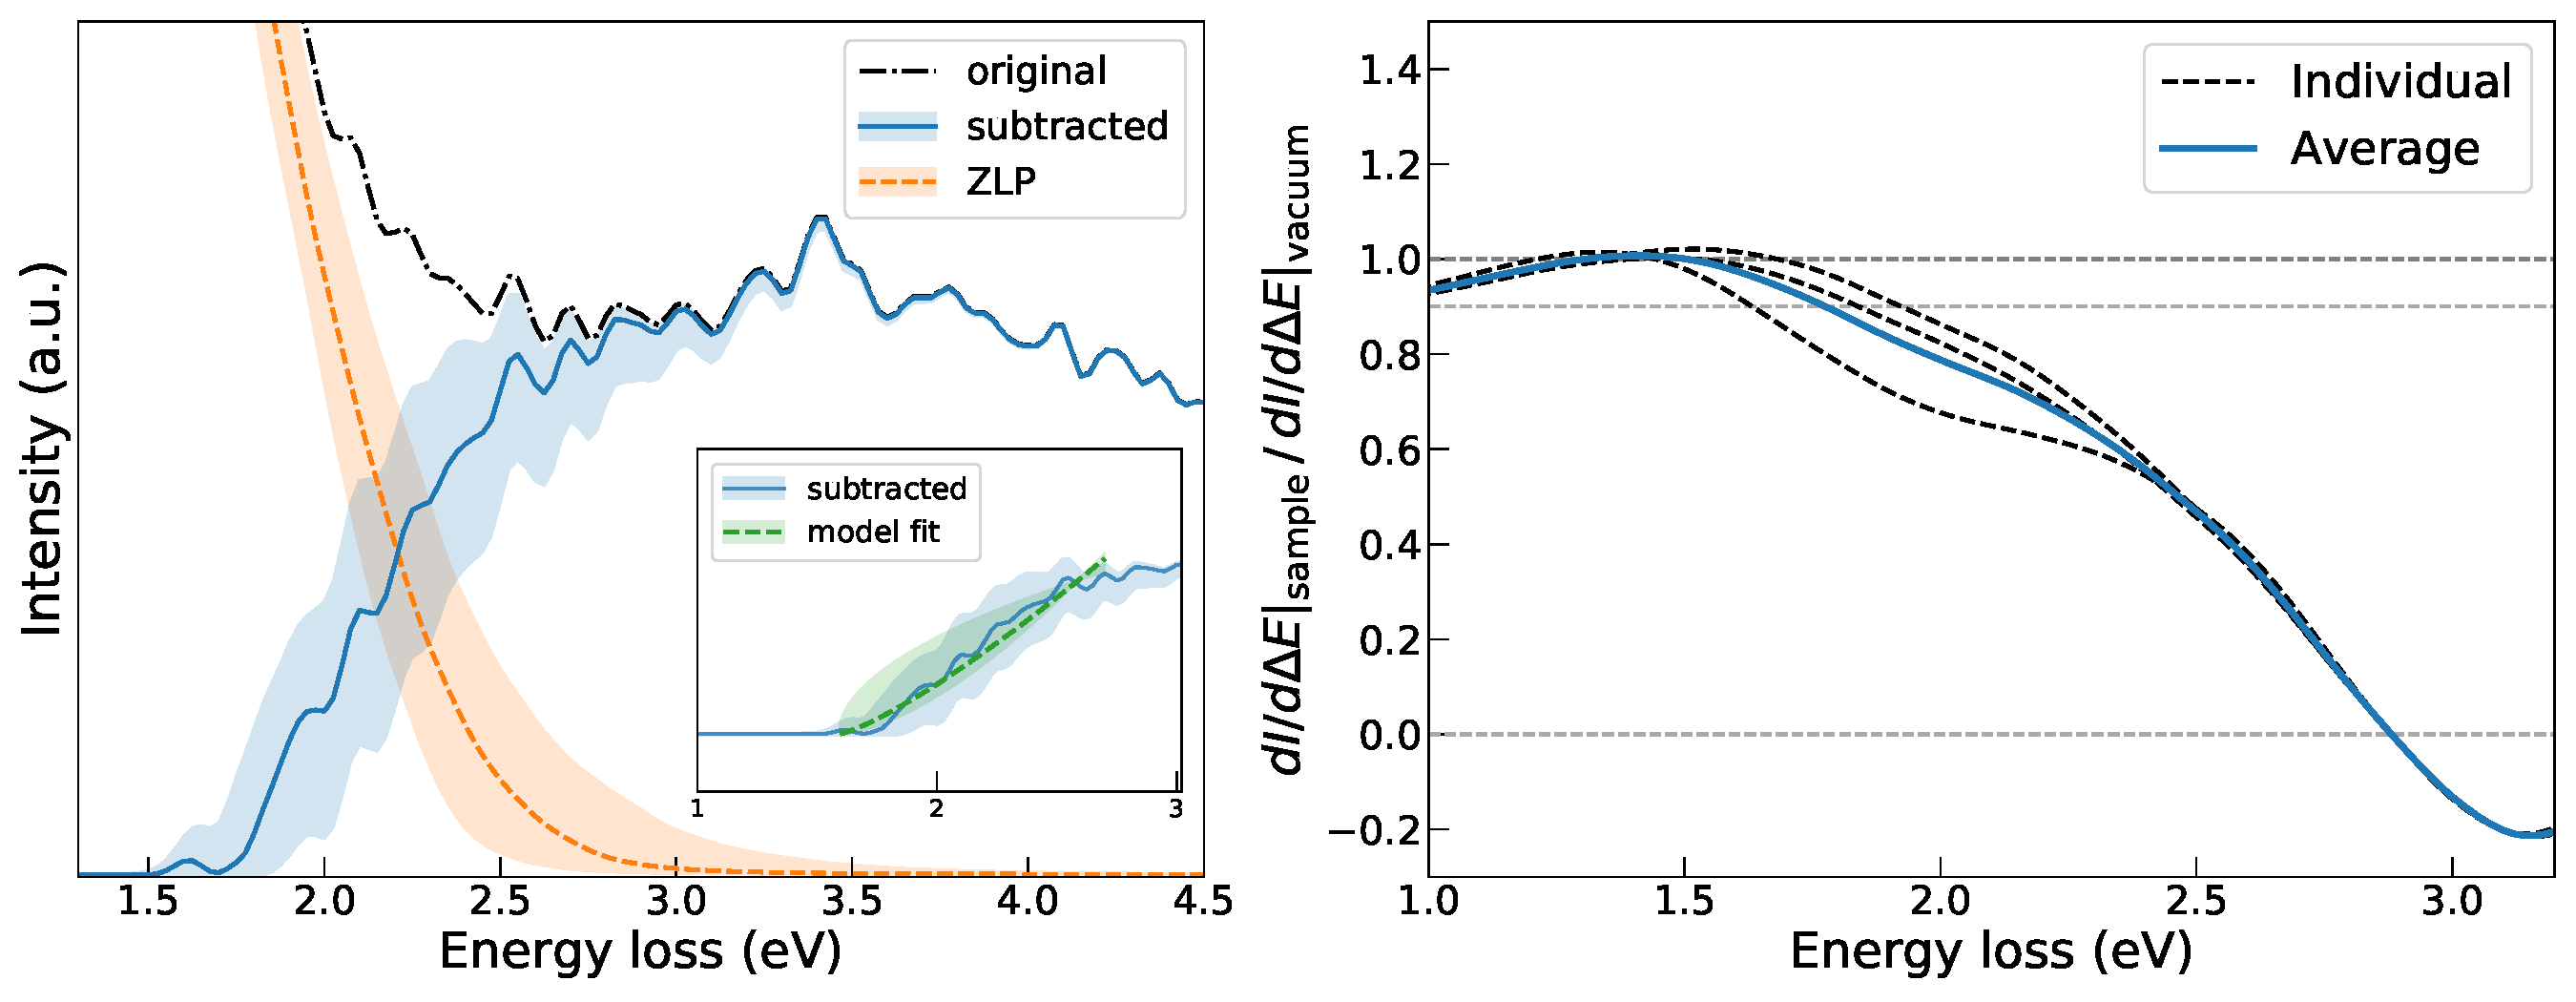
\includegraphics[width=0.99\linewidth]{plots/SubtractedEELS_plot_sp14.pdf}
   \caption{Left: the original
     and subtracted EEL spectrum corresponding to location sp14 of sample A in Fig.~\ref{fig:ws2positions},
     together with the predictions of the ZLP model, where
     the bands indicate the 68\% confidence level uncertainties.
     %
     The inset displays the result of fitting Eq.~(\ref{eq:I1}) to the onset
     region of the subtracted spectrum.
     %
     Right: the ratio of the derivative intensity of the original spectrum, $dI_{\rm EEL}/d\Delta E$,
     over that of the ZLP measurements taken on the vacuum $d I_{\rm ZLP}/d\Delta E$.
  }
\label{fig:sp4_subtracted_spectrum}
\end{centering}
\end{figure}
%%%%%%%%%%%%%%%%%%%%%%%%%%%%%%%%%%%%%%%%%%%%%%%%%%%%%%%%%%%%%%%%%%%%%%%%%%

The inset in the left panel of Fig.~\ref{fig:sp4_subtracted_spectrum}
shows the result of the  fits using Eq.~\ref{eq:I1} to the subtracted spectrum,
with the band indicating the 68\% CL uncertainties.
%
We discuss below the implication of this fit for the bandgap determination
in the WS$_2$ nanostructures.

In the right panel of  Fig.~\ref{fig:sp4_subtracted_spectrum} we display the ratio
between the derivative of the intensity profiles corresponding to the sample locations
with respect to a reference measurement taken on vacuum,
\be
\mathcal{R}_{\rm der}(\Delta E) \equiv 
\frac{
  dI_{\rm EELS}^{(j)}/ d\Delta E
}{
  dI_{\rm EELS}^{(j')} /d\Delta E
}\lp \Delta E\rp \, ,
\ee
where $j'$ labels one of the vacuum spectra.
%
This ratio allows to identify a suitable value of $\Delta E_{I}$ by determining
for which energy losses the derivatives of the sample spectra deviate significantly
from the vacuum ones.
%
Note that $\mathcal{R}_{\rm der}(\Delta E)=0$ indicates the position of the first
local minimum of the spectra.
%
From this comparison we can see that Fig.~\ref{fig:sp4_subtracted_spectrum} validates our choice of
$\Delta E_{\rm I}$.

Fig.~\label{fig:subtracted_spectra_comp} displays the
The ZLP-subtracted spectra corresponding to locations \#4, \#5, and \#6
    in ..... with the corresponding uncertainties.
    %
    Results are shown for two values of the hyperparameter $\Delta E_{\rm I}$,
    1.45 eV (left) and 1.55 eV (right panel).

%%%%%%%%%%%%%%%%%%%%%%%%%%%%%%%%%%%%%%%%%%%%%%%%%%%%%%%%%%%%%%%%%%%%%%%
\begin{figure}[t]
\begin{centering}
  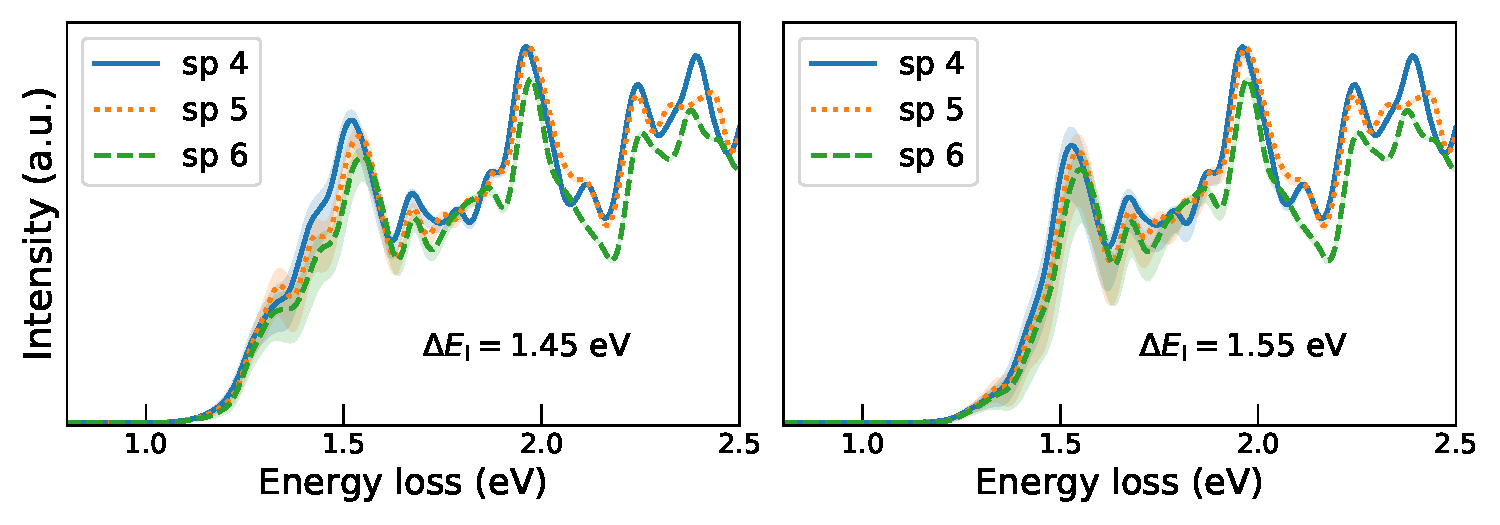
\includegraphics[width=0.99\linewidth]{plots/subtracted_spectra_comp.pdf}
  \caption{The ZLP-subtracted spectra corresponding to locations \#4, \#5, and \#6
    in ..... with the corresponding uncertainties.
    %
    Results are shown for two values of the hyperparameter $\Delta E_{\rm I}$,
    1.45 eV (left) and 1.55 eV (right panel).
  }
\label{fig:subtracted_spectra_comp}
\end{centering}
\end{figure}
%%%%%%%%%%%%%%%%%%%%%%%%%%%%%%%%%%%%%%%%%%%%%%%%%%%%%%%%%%%%%%%%%%%%%%%%%%

\subsection{Bandgap determination}



We now move to discuss the results on the bandgap determination obtained
by fitting the functional form Eq.~(\ref{eq:I1}) to each of the subtracted
spectra defined by Eq.~(\ref{eq:subtractedModelPrediction2}).
%
Results will be presented as a function of the hyper-parameter $\Delta E_{\rm I}$
in order to gauge the stability of the results.
%
To begin with, in Fig.~\ref{fig:bvalues}
we display the values of the bandgap energy $E_{\rm BG}$ (top panels)
and of the exponent $b$ (bottom panels) as a function of $\Delta E_I$
for locations \#4 (left)
and \#5 (right panels) from Sample A indicated in Fig.~\ref{fig:ws2positions}.
%
The central value and the error band for each value of $\Delta E_I$ is evaluated
as the median and the 68\% CL interval over the $N_{\rm rep}=500$ Monte Carlo replicas.
%
The red marker indicates the position of the optimal value of
$\Delta E_{\rm I}$ determined as specified above.

%%%%%%%%%%%%%%%%%%%%%%%%%%%%%%%%%%%%%%%%%%%%%%%%%%%%%%%%%%

\begin{figure}[t]
\begin{centering}
  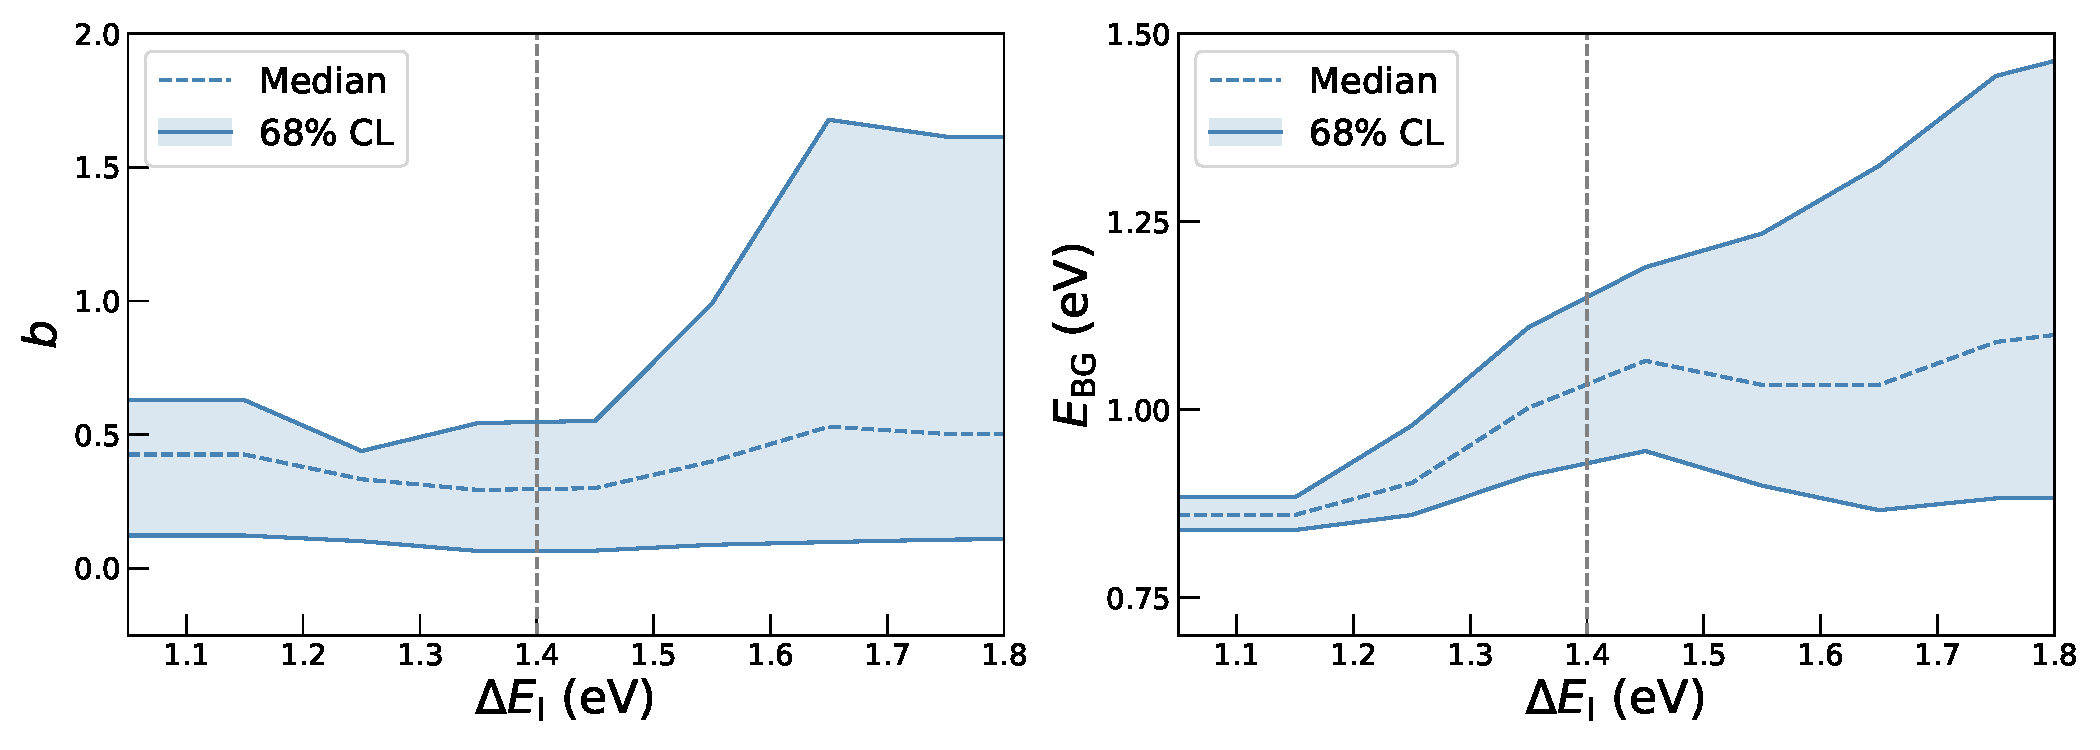
\includegraphics[width=0.6\linewidth]{plots/Stability_plots_sp4.pdf}
  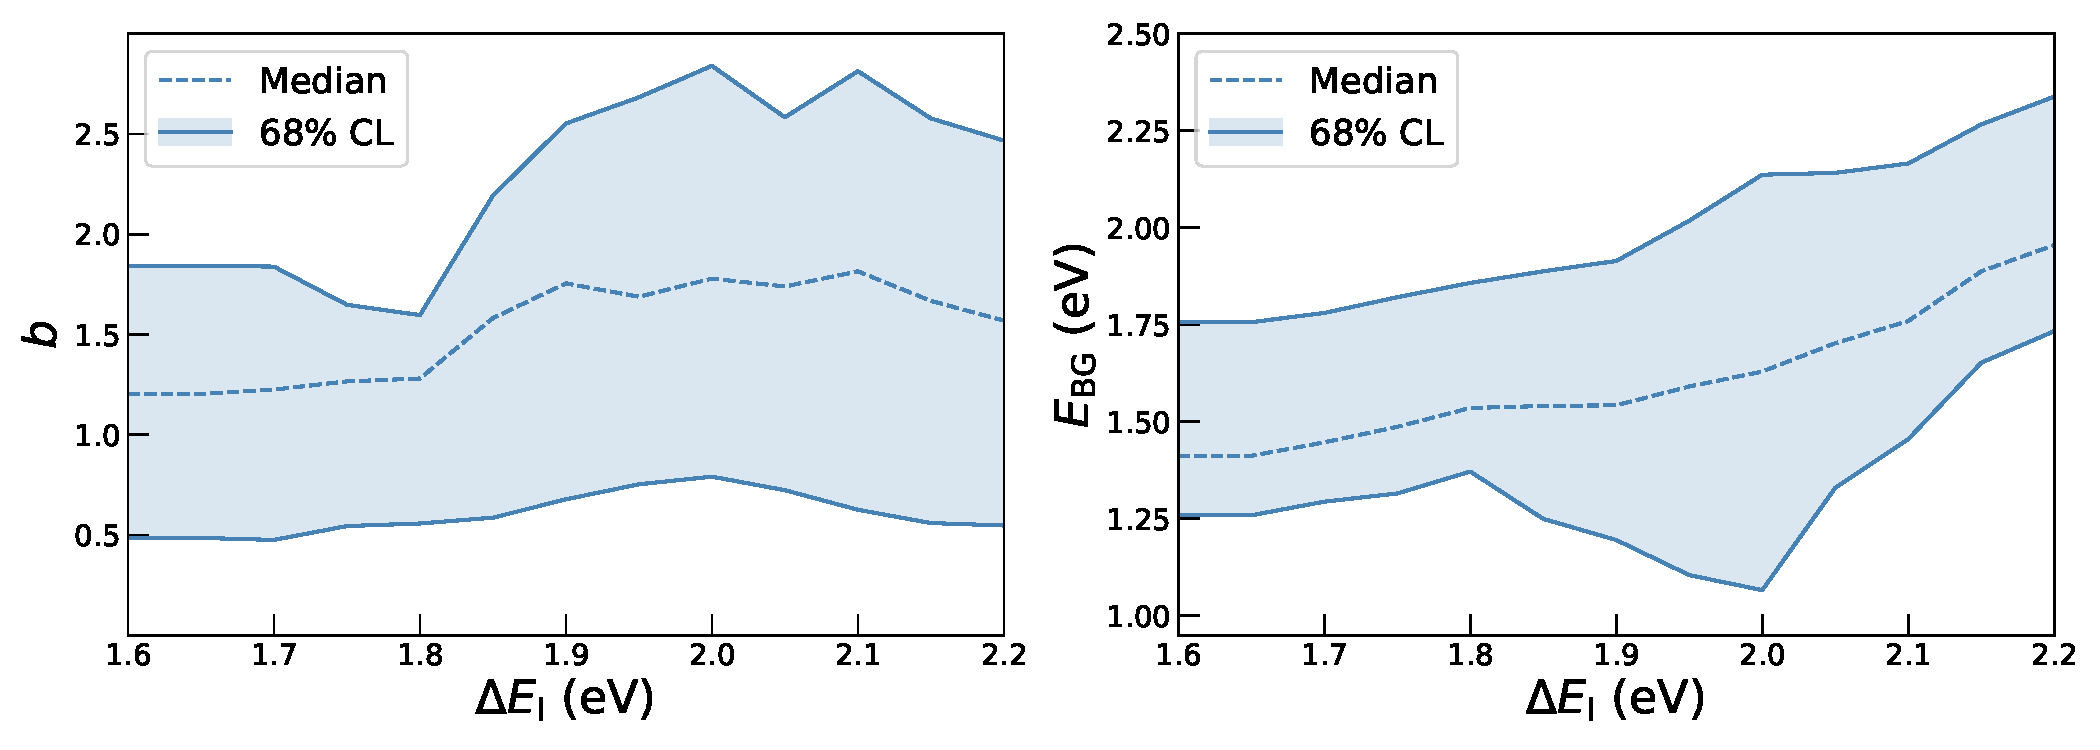
\includegraphics[width=0.6\linewidth]{plots/Stability_plots_sp14.pdf} 
  \caption{Top: the values of the bandgap energy $E_{\rm BG}$ and of the exponent $b$
  obtained from fits to the onset
  region of subtracted spectra using Eq.~(\ref{eq:I1}) as a function
  of the hyper-parameter $\Delta E_{\rm I}$.
  %
  We show results for locations \#4 from set A (top)
  and \#14 of set B (bottom) indicated in Fig.~\ref{fig:ws2positions}.
  %
  The central value and the error band for each value of $\Delta E_I$ is evaluated
  as the median and the 68\% CL interval over the $N_{\rm rep}=500$ Monte Carlo replicas.
  }
\label{fig:bvalues}
\end{centering}
\end{figure}
%%%%%%%%%%%%%%%%%%%%%%%%%%%%%%%%%%%%%%%%%%%%%%%%%%%%%%%%%%%%%

In Table~\ref{table:bandgap_fitting} we collect
 the median values and 68\% CL ranges for the bandgap energy $E_{\rm BG}$
 and the bandgap exponent $b$ determined from fitting Eq.~(\ref{eq:I1}) to each of the subtracted
 spectra defined by Eq.~(\ref{eq:subtractedModelPrediction2}).
 %
 We consider two representative spectra from sample A and two
 from sample B. 
 %
 The error is divided into the statistical and the systematic component, which are
 then added in quadrature to evaluate the total uncertainty in the fit results. 
 %
 From these results we see that the spectra in sample A are consistent with a direct bandgap,
 while those of sample B with an indirect bandgap.

%%%%%%%%%%%%%%%%%%%%%%%%%%%%%%%%%%%%%%%%%%%%%%%%%%%%%%%%%%%%%%%%%%%%%%%%%%%%%%%%%%%%%%%%%%%%%
%%%%%%%%%%%%%%%%%%%%%%%%%%%%%%%%%%%%%%%%%%%%%%%%%%%%%%%%%%%%%%%%%%%%%%%%%%%%%%%%%%%%%%%%%%%%%
\begin{table}[t]
  \begin{center}
    \footnotesize
            \renewcommand{\arraystretch}{1.50}
  \begin{tabular}{@{}c|c|c|c}
\br
Set & Spectrum   &$E_{\rm BG}$~(eV)  &  $b$  \\
\mr
\mr
A        &   sp\#4   &     $ 2.0 \pm 0.3^{\rm (stat)} \pm  0.2^{\rm (sys)}=  2.0 \pm 0.3^{\rm (tot)}   $                &       $ 0.5 \pm 0.3^{\rm (stat)} \pm  0.2^{\rm (sys)}=  0.5 \pm 0.3^{\rm (tot)}   $                       \\
\mr
A        &   sp\#5   &     $ 2.0 \pm 0.3^{\rm (stat)} \pm  0.2^{\rm (sys)}=  2.0 \pm 0.3^{\rm (tot)}   $                &       $ 0.5 \pm 0.3^{\rm (stat)} \pm  0.2^{\rm (sys)}=  0.5 \pm 0.3^{\rm (tot)}   $                       \\
\mr
\mr
B        &   sp\#14   &     $ 2.0 \pm 0.3^{\rm (stat)} \pm  0.2^{\rm (sys)}=  2.0 \pm 0.3^{\rm (tot)}   $                &       $ 0.5 \pm 0.3^{\rm (stat)} \pm  0.2^{\rm (sys)}=  0.5 \pm 0.3^{\rm (tot)}   $                       \\
\mr
B        &   sp\#15   &     $ 2.0 \pm 0.3^{\rm (stat)} \pm  0.2^{\rm (sys)}=  2.0 \pm 0.3^{\rm (tot)}   $                &       $ 0.5 \pm 0.3^{\rm (stat)} \pm  0.2^{\rm (sys)}=  0.5 \pm 0.3^{\rm (tot)}   $                       \\
\br
  \end{tabular}
    \end{center}
  \caption{\small The median values and 68\% CL ranges for the bandgap energy $E_{\rm BG}$
    and the bandgap exponent $b$ determined from fitting Eq.~(\ref{eq:I1}) to each of the subtracted
    spectra defined by Eq.~(\ref{eq:subtractedModelPrediction2}).
    %
    As justified in the text, we consider two representative spectra from sample A and two
    from sample B. 
    %
    The error is divided into the statistical and the systematic component, which are
    then added in quadrature to evaluate the total uncertainty in the fit results. {\rm ToDo}.
  }
   \label{table:bandgap_fitting}
\end{table}
%%%%%%%%%%%%%%%%%%%%%%%%%%%%%%%%%%%%%%%%%%%%%%%%%%%%%%%%%%%%%%%%%%%%%%%%%%%%%%%%%%%%%%%%%%%%%%%%%5
%%%%%%%%%%%%%%%%%%%%%%%%%%%%%%%%%%%%%%%%%%%%%%%%%%%%%%%%%%%%%%%%%%%%%%%%%%%%%%%%%%%%%%%%%%%%%
